\documentclass[11.5pt,a4paper,russian]{article}
\usepackage[utf8]{inputenc}
\usepackage[T1,T2A]{fontenc}
\usepackage{indentfirst}
\usepackage[russian]{babel}
\usepackage[a4paper]{geometry}
\geometry{verbose,tmargin=1cm,lmargin=1cm,rmargin=1cm, bmargin=2cm}
\usepackage{float}
\usepackage{amsbsy}
\usepackage{amsmath}
\usepackage{setspace}
\usepackage{amsmath}
\usepackage{wrapfig}
\usepackage{booktabs}
\usepackage{caption}
\usepackage{subcaption}
\usepackage{graphicx}
\graphicspath{ {images/} }

\begin{document}

\begin{titlepage}

\begin{center}

\large \textit{\small Московский физико-технический институт (государственный университет)}

\vspace{5cm}
\textit{Работа 5.5.2}

\vspace{1cm}
\textbf{\huge Спектрометрия $\alpha$-излучения с помощью полупроводникового детектора}

\vspace{12cm}

\begin{flushright}
\parbox{0.45\textwidth}{
Выполнил: \\[0.5cm]
Киракосян Давид Арсенович (Б02-006) \\[0.2cm]
}
\end{flushright} 

\vfill

\today
\end{center}
\end{titlepage}

\textbf{Цель Работы:}  C помощью кремниевого поверхностно-барьерного детектора измеряются спектры $\alpha$-частиц, испускаемых различными радиоактивными ядрами - ${ }^{226} \mathrm{Ra},{ }^{238} \mathrm{U},{ }^{241} \mathrm{Am} + ^{230} \mathrm{Th}$ и ${ }^{239} \mathrm{Pu}$. Исследуется тонкая структура $\alpha-$ излучения и последовательность радиоактивных распадов в семействе урана.

\section{Теоретические сведения}
К числу радиоактивных процессов относятся $\alpha$- и $\beta$-распады (в том числе и $K$-захват), $\gamma$-излучение, деление ядер, а также испускание запаздывающих нейтронов и протонов. В этой работе изучается $\alpha$-распад.\\
Энергию вылетающих из ядра $\alpha$-частиц легко подсчитать на основе законов сохранения. Если родительское (исходное) ядро имеет массу $M_1$, а дочернее (конечное) - $M_2$, то законы сохранения энергии и импульса записываются в форме

$$
\begin{gathered}
M_2 c^2=M_1 c^2+m_\alpha c^2+T_1+T_\alpha, \\
\mathrm{p}_1+\mathrm{p}_\alpha=0
\end{gathered}
$$

где $T_1$ и $\mathrm{p}_1$ - кинетическая энергия и импульс отдачи дочернего ядра, a $T_\alpha$ и $\mathrm{p}_\alpha$ - кинетическая энергия и импульс $\alpha$-частицы.

Ясно, что вылет $\alpha$-частицы из ядра возможен лишь в том случае, если разность энергий покоя родительского и дочернего ядра будет больше энергии покоя $\alpha$-частицы. В силу того, что реально $\alpha$-распад испытывают лишь тяжелые ядра с $A>200$, энергия отдачи ядра очень мала и фактически кинетическая энергия $\alpha$-частицы равна разности энергий покоя исходного и конечного ядер. Именно поэтому вылетающие $\alpha$-частицы имеют строго определенную энергию.

Однако экспериментально обнаружено, что энергетический спектр $\alpha$-частиц многих $\alpha$-активных ядер состоит из нескольких линий, одна из которых преобладающее. Дискретность линий и их относительная интенсивность объяснимы, поскольку, во-первых, $\alpha$-частицы могут испускаться ядром, находящимися в возбужденном состоянии (длиннопробежные $\alpha$-частицы), а во-вторых может происходить $\alpha$-распад из основного состояния родительского ядра на возбужденные состояния дочернего ядра (короткопробежные $\alpha$-частицы). Так как период полураспада для $\alpha$-частиц примерно в $10^5$ раз больше периода $\alpha$-распада, то интенсивность длиннопробежных $\alpha$-частиц очень мала.

Тяжелые ядра, как правило, в основном состоянии деформированы (исключением являются магические ядра). Это означает, что низколежащими состояниями являются вращательные полосы, и именно на эти состояния обычно и происходит распад родительского ядра, приводящий к появлению группы короткопробежных $\alpha$-частиц. Как известно, энергия вращательных уровней определяется выражением

$$
E_\text{вp}=\frac{\hbar^2}{2 \mathcal{I}} l(l+1).
$$

Тем самым измерение тонкой структуры энергетического спектра $\alpha$ частиц дает возможность определить момент инерции ядра $\mathcal{I}$.

Периоды полураспада $\alpha$-активных ядер очень сильно зависят от энергии вылетающих частиц. Экспериментально установленная зависимость (закон Гейгера-Нэттола) имеет вид:

\begin{equation}\label{eq:gey_net}
\lg T_{1 / 2}=\frac{a}{\sqrt{E_\alpha}}+b .
\end{equation}

Коэффициенты $a$ и $b$ очень слабо зависят от заряда ядра $Z$.

\section{Экспериментальная установка}
В состав экспериментальной установки входит альфа-спектрометр, форвакуумный насос и персональный компьютер. (Рис. \ref{fig:scheme})

\begin{figure}[h]
  \centering
  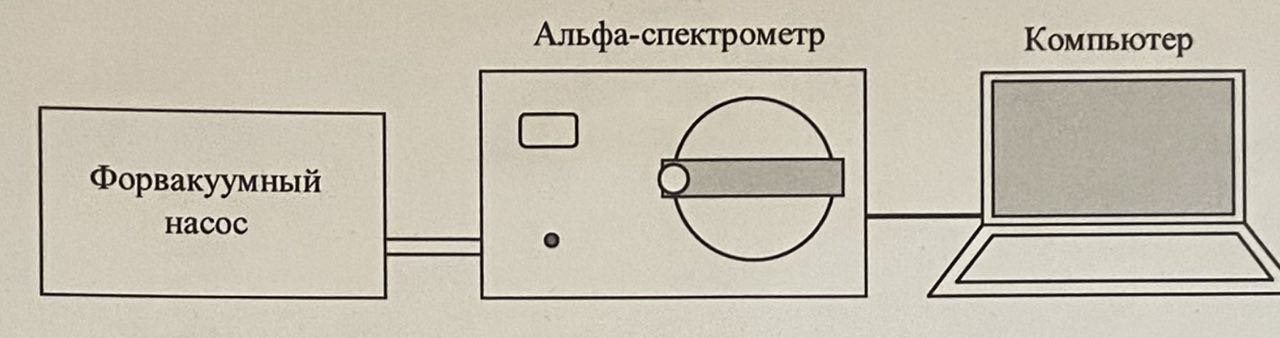
\includegraphics[width=0.8\textwidth]{710a8508-9868-4ef0-989c-5313e27d6a45}  \caption{Блок-схема спектрометра $\alpha$-излучения}
  \label{fig:scheme}
\end{figure}

Форвакуумный насос, соединенный с корпусом альфа-спектрометра вакуум-ным шлангом, откачивает измерительную камеру до давления 0,2 мм рт. ст.\\
Установка автоматически поддерживает давление в измерительной камере в рабочем диапазоне от 0,2 до 2,0 мм рт. ст. Откачка блокируется при разгер-метизации камеры. Соединение и отсоединение измерительной камеры с атмосферой осуществляется с помощью двух электромагнитных клапанов.\\
Внешний вид альфа-спектромерта изображен рис \ref{fig:spectrometer}а.

\begin{figure}[h]
  \centering
  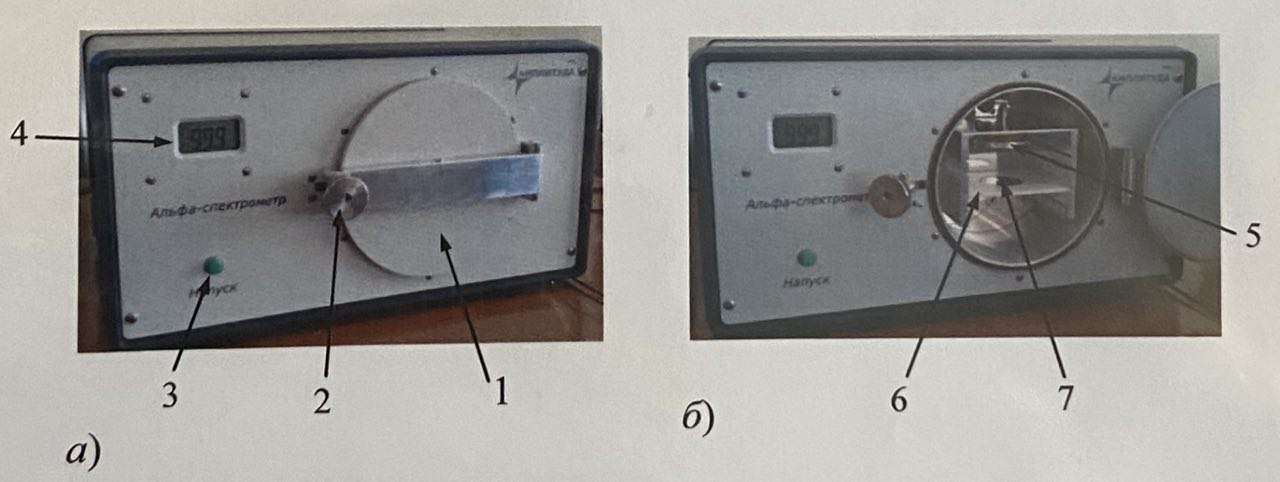
\includegraphics[width=0.8\textwidth]{1447354b-08af-499c-9336-bcffb286f7cc}  \caption{Блок-схема спектрометра $\alpha$-излучения}
  \label{fig:spectrometer}
\end{figure}

Здесь 1 - крышка измерительной камеры, 2 - прижимная ручка, 3 - кнопка разгерметизации (напуска атмосферы), 4 - индикатор давления в камере (показывает давление в мм рт. ст.). Внутри измерительной камеры альфа-спектрометра (рис. 26) располагается полупроводниковый детектор 5, держатель образца 6 вместе с металлической подложкой 7, на которую устанавливают образцы с радиоактивными источниками. Металлическая подложка 7 соединена гибким проводником с источником постоянного напряжения. На подложку 7 подается отрицательный потенциал (относительно корпуса измерительной камеры) для того, чтобы ядра отдачи, получившие импульс, направленный вверх, не попадали на детектор и не загрязняли его. Держатель образца 6 вместе с самим образцом можно располагать на нескольких фиксированных расстояниях от детектора. Электрический сигнал с полупроводникового детектора усиливается, поступает на плату аналогово-цифрового преобразователя (АЦП) и обрабатывается компьютером.

Амплитуда электрического сигнала с полупроводникового детектора пропорциональна энергии а - частицы, и поэтому с помощью компьютера мы регистрируем спектры источников. Осуществляется это с помощью установленной на компьютере программы "Прогресс"

При использовании детектора в спектрометрических целях особое значение приобретает его разрешающая способность, т. е. ширина кривой распределения импульсов по амплитудам при строго постоянной энергии регистрируемых частиц. Форма такой кривой распределения обычно бывает близка к кривой ошибок (гауссовой кривой)

$$
W(U) d U=\frac{1}{\sqrt{2 \pi} \sigma} e^{-\left(U-U_0\right)^2 /\left(2 \sigma^2\right)} d U
$$

Распределение (5) имеет вид колокола с максимумом при $U=U_0$. Разрешающую способность спектрометра определяют по величине $\delta$ ширине кривой $W(U)$, измеренной на половине высоты. Энергетическим разрешением спектрометра обычно называют величину

$$
R=\frac{\delta}{U_0} \cdot 100 \% .
$$

Нетрудно найти связь между $\delta$ и б:

$$
\delta=2 \sqrt{2 \ln 2} \sigma .
$$

Одной из основных причин, вызывающих разброс импульсов по амплитуде, является статистическая флуктуация числа электрондырочных пар, создаваемых падающей частицей. Среднее число пар $N$ равно

$$
N=E / E_{\mathrm{cp}},
$$

где $E$ - энергия, теряемая частицей в детекторе, а $E_{\mathrm{cp}}=3.6$ эВ - энергия, необходимая для создания пары электрон-дырка. Среднеквадратичное отклонение $\sigma$ равно

$$
\sigma=\sqrt{N}=\sqrt{E / E_{\mathrm{cp}}}
$$

Вклад флуктуаций числа пар в энергетическое разрешение

$$
R_{\text {флук }}=\frac{\sigma}{N} \cdot 100 \%=\sqrt{\frac{E_{\mathrm{cp}}}{E}} \cdot 100 \% .
$$

\section{Ход Работы}
Получим зависимость счета на сцинтилляторе $N'_\text{ч}$ от номера канала $N$ для разных веществ: ${}^{226}\mathrm{Ra},{}^{238}\mathrm{U}, { }^{239} \mathrm{Pu}$, ${}^{241}\mathrm{Am} + ^{230} \mathrm{Th}$. Спектр ${ }^{226} \mathrm{Ra}$ будем использовать для калибровки горизонтальной оси. Найдем номера пиков:

\begin{equation}\label{}
	N_1 = 1594.7, \quad N_2 = 1828.2, \quad N_3 = 1998.1, \quad N_4 = 2540.2
\end{equation}

Мы знаем, что этим пикам соответствуют табличные значения энергии $4.784, 5.490$, $6.002, 7.687$ МэВ соответственно. Тогда проведем калибровку спектрометра, построив линейную зависимость энергии гамма-кванта от номера канала $E_i = f(N_i)$ (Рис. \ref{fig:calib}). Результат калибровки:

\begin{equation}
	E_i = (-0.1267 + 0.0031N_i ) \; \text{МэВ}
\end{equation}
\begin{figure}[h!]
\centering
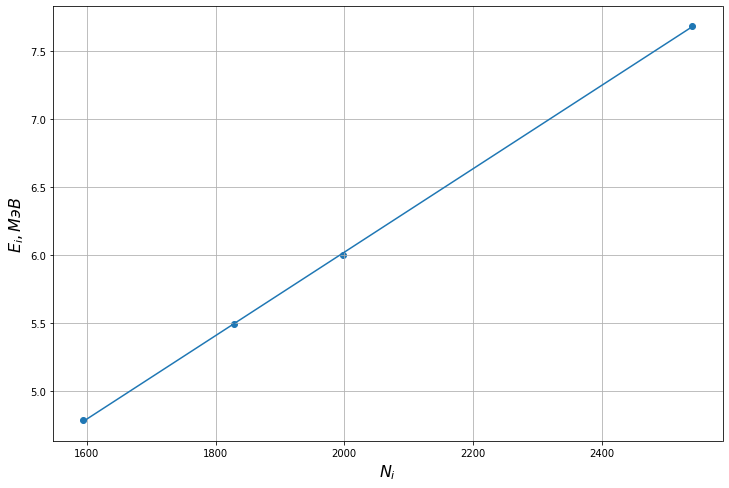
\includegraphics[width=0.65\textwidth]{05cdfd8e-505f-4549-8864-26c91e3d9761}
\caption{Калибровочный график $E_i = f(N_i)$}
\label{fig:calib}
\end{figure}

С помощью полученной зависимости переведем все полученные значения каналов в энергии, а счет сцинтиллятора не будем отнормировать по времени, так как все измерения были проведены за $600 \pm 3$ секунды. Также занесем значения максимумов в таблицу \ref{table:energy}

\begin{figure}[h!]
\centering
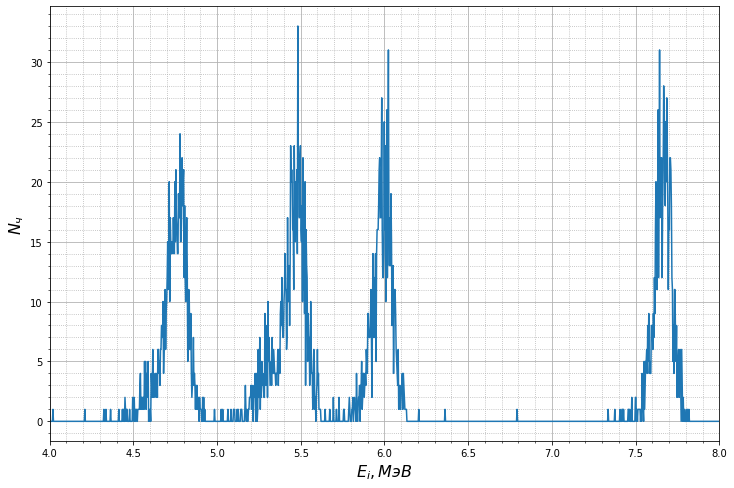
\includegraphics[width=0.7\textwidth]{c199c04d-a769-427b-b585-fb9c75c84bc0}
\caption{Спектр ${ }^{226} \mathrm{Ra}$}
\end{figure}

\begin{figure}[h!]
\centering
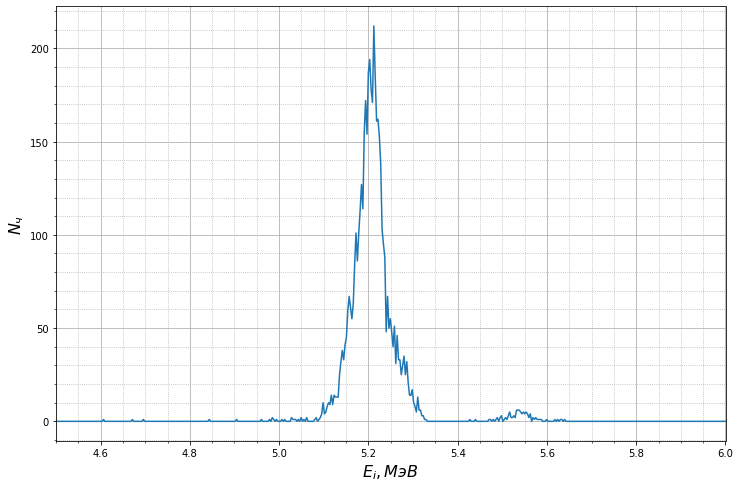
\includegraphics[width=0.7\textwidth]{44b70cf4-4b6c-48fa-825a-fe3d68087e3e}
\caption{Спектр ${ }^{239} \mathrm{Pu}$}
\end{figure}


\begin{figure}[h!]
\centering
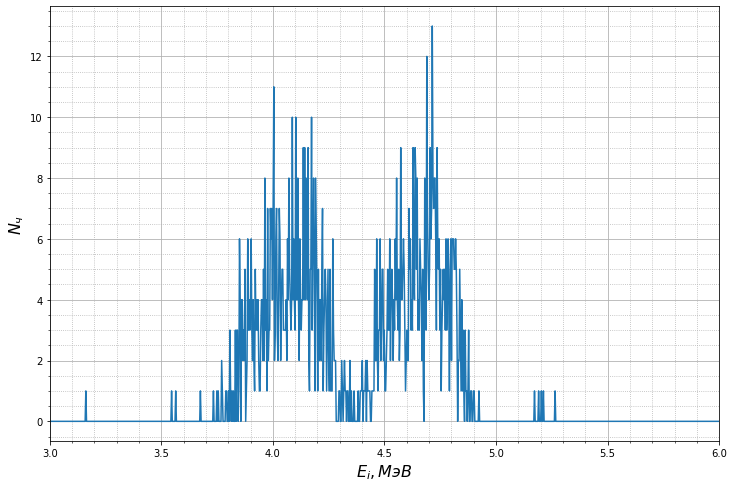
\includegraphics[width=0.7\textwidth]{d85fc747-d9e2-4576-84f2-54f3d4065373}
\caption{Спектр ${ }^{238} \mathrm{U}$}
\end{figure}

\begin{figure}[h!]
\centering
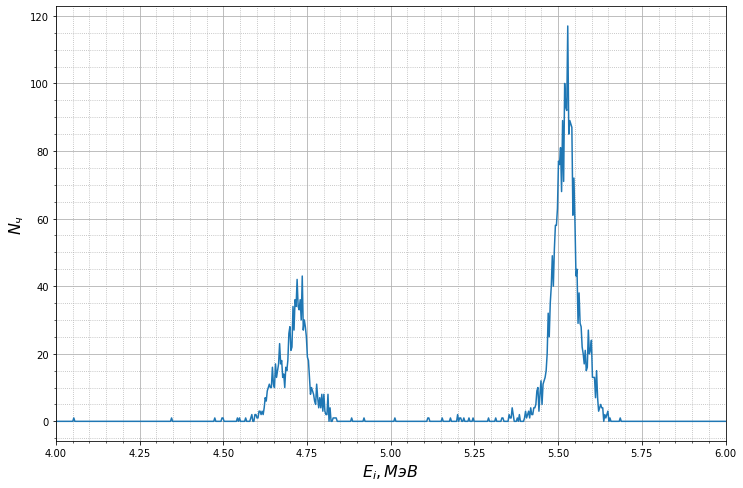
\includegraphics[width=0.7\textwidth]{5f5f271d-9b7a-45db-9c74-f1768a235b47}
\caption{Спектр ${ }^{241} \mathrm{Am} + ^{230} \mathrm{Th}$}
\end{figure}

\begin{table}[h!]
  \centering
  \caption{Пики $\alpha$-спектров}
\begin{tabular}{l|c|c|c|c|c|c}
\toprule 
Образец & $N_i$ & $\Delta N_i$ & $E_i$ & $\Delta E_i$ & $R_i$ & $R_\text{фл}, 10^{-4}$ \\
\midrule ${ }^{239} \mathrm{Pu}$ & 1738.639 & 18.063 & 5.217 & 0.056 & 0.010 & 8.31 \\
${ }^{239} \mathrm{Pu}$ (доч.) & 1845.025 & 12.345 & 5.544 & 0.038 & 0.007 & 8.06 \\
${ }^{226} \mathrm{Ra}$ & 1594.688 & 30.224 & 4.775 & 0.093 & 0.019 & 8.68 \\
${ }^{226} \mathrm{Ra}$ (доч.) & 1828.164 & 26.150 & 5.492 & 0.080 & 0.014 & 8.10 \\
${ }^{226} \mathrm{Ra}$ (доч.) & 1998.108 & 23.183 & 6.015 & 0.071 & 0.012 & 7.74 \\
${ }^{226} \mathrm{Ra}$ (доч.) & 2540.184 & 24.510 & 7.681 & 0.075 & 0.010 & 6.85 \\
${ }^{241} \mathrm{Am} + ^{230} \mathrm{Th}$ & 1581.102 & 17.973 & 4.733 & 0.055 & 0.011 & 8.72 \\
${ }^{241} \mathrm{Am} + ^{230} \mathrm{Th}$ (доч.) & 1841.891 & 18.608 & 5.535 & 0.057 & 0.010 & 8.07 \\
${ }^{238} \mathrm{U}$ & 1388.365 & 49.676 & 4.141 & 0.153 & 0.036 & 9.32 \\
${ }^{238} \mathrm{U}$ (доч.) & 1566.426 & 69.002 & 4.688 & 0.212 & 0.044 & 8.76 \\
\bottomrule
\end{tabular}
  \label{table:energy}
\end{table}

Для ${ }^{226} \mathrm{Ra}$ разница $R_i - R_\text{фл} = 0.01$.

Построим теперь зависимость $T_{1/2}(1/\sqrt{E_\alpha})$, для проверки закона Гейгера-Нетолла (\ref{eq:gey_net}). Времена полураспада ${ }^{226} \mathrm{Ra}$ и дочерних ядер приведены в таблице \ref{table:gey_net}. График представлен на Рис. \ref{fig:gey_net}.

\begin{table}[h!]
\centering
\caption{Время полураспадов ${ }^{226} \mathrm{Ra}$ и дочерних ядер}
\label{table:gey_net}
\begin{tabular}{l|c|c|c|c}
\toprule
Образец & ${ }^{226}_{88} \mathrm{Ra}$ & ${ }^{222}_{86} \mathrm{Rn}$ & ${ }^{218}_{84} \mathrm{Po}$ & ${ }^{214}_{84} \mathrm{Po}$ \\
\midrule
    $T_{1/2}$ & 1620 лет & 3.82 суток & 3.11 мин. & $1.63 10^{-4}$ сек. \\
\bottomrule
\end{tabular}
\end{table}

\begin{figure}[h!]
  \centering
  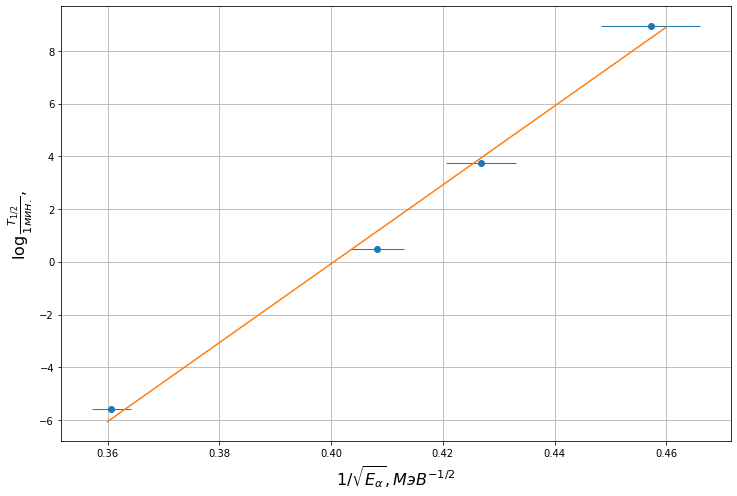
\includegraphics[width=0.7\textwidth]{ea5bb392-4357-4db4-853a-a0e22ec27231}  \caption{Проверка закона Гейгера-Нетолла}
  \label{fig:gey_net}
\end{figure}

\newpage
\section{Вывод}
В ходе работы были проведены измерения спектров $\alpha$-излучения, были получены энергии $\alpha$-распадов для разных веществ, которые приведены в таблице \ref{table:energy}. Также был проверен закон Гейгера-Нетолла связывающий период полураспада с энергией излучения.


\end{document}